\documentclass[a4paper]{article}
\usepackage{sst2022,amssymb,amsmath,epsfig,lipsum}
\usepackage[hidelinks]{hyperref}
\setcounter{page}{1}
\sloppy     % better line breaks
\ninept
%SM below a registered trademark definition
\def\reg{{\rm\ooalign{\hfil
     \raise.07ex\hbox{\scriptsize R}\hfil\crcr\mathhexbox20D}}}


%% \newcommand{\reg}{\textsuperscript{\textcircled{\textsc r}}}
\title{NFT as a proof of Digital
Ownership-reward system integrated to a
Secure Distributed Computing Blockchain
Framework}

%%%%%%%%%%%%%%%%%%%%%%%%%%%%%%%%%%%%%%%%%%%%%%%%%%%%%
%% If multiple authors, uncomment and edit the lines shown below.       %%
%% Note that each line must be emphasized {\em } by itself.             %%
%% (by Stephen Martucci, author of spconf.sty).                         %%
%%%%%%%%%%%%%%%%%%%%%%%%%%%%%%%%%%%%%%%%%%%%%%%%%%%%%
%\makeatletter
\def\name#1{\gdef\@name{#1\\}}
%\makeatother
%\name{{\em %Lastname1, Firstname2 Lastname2, Firstname3 Lastname3,}\\
%      {\em Firstname4 Lastname4, Firstname5 Lastname5, Firstname6 Lastname6,
%      Firstname7 Lastname7}}
%%%%%%%%%%%%%%% End of required multiple authors changes %%%%%%%%%%%%%%%%%

\makeatletter
\def\name#1{\gdef\@name{#1\\}}
\makeatother \name{{\em Asahi Cantu}}

\address{University of Stavanger\\
{\small \tt asahicantu@outlook.com}}

%
\begin{document}
\maketitle
%
\begin{abstract}
Today, the global economy is dependent on the Internet and computational resources. Although they are tightly interconnected, it is difficult to evaluate their
degree of interdependence. Keeping up with the pace of technology can be a challenging task, mainly when updating the hardware and software infrastructure. Every day, corporations and governments are faced with this issue; most have been
victims of cyber attacks, security breaches, and data leaks. The consequences are
significant in monetary losses; damage remediation is unattainable, even impossible, in certain circumstances. The repercussions might include reputational damage, legal responsibility, and threats to national security (when attacks are carried
out against critical infrastructures to control the resources of a country), to name a
few. Similarly, data has become such an integral part of many industries that it is
one of the most critical targets for attackers that often is encrypted by ransomware,
stolen, or corrupted. Without data, many companies are not be able to continue
operating as they do. The combination of all these factors complicates the ability
of organizations to cooperate, trust, and share information in efforts to research
and develop solutions for industry and government.
A promising technology can assist in significantly reducing the damage caused
by the security threats outlined above: Blockchain technology has proven to be one
of the most promising inventions of the twenty-first century for transmitting and
protecting information while offering high reliability and availability, low exposure
to attacks, protected encrypted data, and accessible to the entities willing to participate. Blockchain enabled the possibility to embed immutable data and compiled
source code known as ‘smart contract’ where certain rules can be programmed to
create business workflows.
This work proposes a Blockchain-based infrastructure solution provided by ”Hyperledger Fabric” technology for companies to securely transmit and
share information using the latest encryption and data storage technologies operating on the model of distributed systems and smart contracts. By presenting
unique digital assets as Non-Fungible Tokens (NFT), the infrastructure is able to
trust the integrity of the data, while protecting it from counterfeiting. Through the
use of a Blockchain-based file storage system known as IPFS, and by connecting all
the relevant elements together through a web-based application, it is possible to
demonstrate that the implementation of such systems is feasible, highly scalable
and a useful tool that many organizations can utilize to create new work systems
and workflows for digital asset management.
 \end{abstract}
\noindent{\bf Index Terms}: blockchain, hyperledger, hyperledger fabric, NFT, permissioned blockchain, tokens, react, web, fullstack, secure, trustless, decentralized, IPFS, DFS, ERC-721

%
\section{Introduction}
As Blockchain technologies attract the interest of worldwide industries for its intrinsic values, new possibilities unleash to promote mutual cooperation in benefit of building up and improving technologies securely and manageable\cite{nakamoto2008bitcoin}. Companies can benefit from such systems when through inter-organizational trust, privacy and protection; improving and protecting businesses while cooperating and sharing information through a common system.
When it comes to large-volume data sharing and storage, it becomes vital to verify its authenticity and avoid plagiarism/counterfeiting. The project proposes a system for the treatment of data as a digital asset through the concept of smart contracts\cite{ERCEther92:online} to manage Non-fungibility in a Blockchain system, and a server/application infrastructure to expose the potential and possibilities that data ownership can have when it is brought into decentralized permissioned systems with Hyperledger Fabric as a Blockchain system and Interplanetary File System (IPFS)
as a Distributed File System (DFS) system.

The digital era keeps evolving and cloud computing increases its power, users and companies are no longer in full control of their resources, rather than that, they led third party companies to store their information without fully knowing the way or locations it could be. In addition to this, recent cyber security risks and the progress of malware, ransomware and other harmful technologies have put the whole world into a cyber crisis. Ever since the creation of the interned such cyber attacks have been increasing exponentially and represent risks for the assets of the companies, countries and end users. Data is vital, data keeps breaching and leaking sometimes without event noticing but months after the damage has happened. 

This brings the need for an implementation of a more secure way to store and manage data through the internet without suffering from the present security risks.

Decentralized systems and Blockchain technologies created in the last ten years offer a tremendous potential to bring organization into a new way to manage their virtual assets. 

It is therefore the purpose of this project to create an architecture and functional system to record unique ownership of digital assets in a permissioned blockchain (datasets ownership) while providing the infrastructure to allow its usage or deny it depending on the agreements of the system through the issuance of NFT's and smart contracts as an alternative solution that allows to alleviate the present cyber security risks while enabling data management securely and privately.

\section{Approach}
This is work uses Hyperledger Fabric permissioned Blockchain framework as a base platform to implement an ERC-721 smart contract extension for the creation and certification of digital assets, which for the aim of this work is represented in data. 
It also implements an distributed data lake infrastructure through the usage of a private IPFS network, which allows storage of information in a reliable and trustless manner. When this data is linked to the ERC-721 smart contract, an NFT asset is created, and single entity properties like ownership, authenticity, transfer, royalties, etc, can be exposed to all its participants.

It demonstrate through the creation of a back-end and front-end example applications the potential of its usage through a simulated token minting and data sharing environment among different known parties where the unique source of trust is a central authority and the previous agreement of the rules (consensus protocol) through which the data can be generated, shared and transferred in the same manner as if a crypto asset was transferred. Since the environment has been implemented using Docker Containers Technology, its scalability and security are granted and can be easily implemented.  The results can be visualized in  the following github repository, the program can be downloaded and deployed in any computer system with specific requirements
\begin{itemize}
    \item ERC-721 protocol creation and extension
    \item Consensus mechanism
    \item Infrastructure and Blockchain environment in Hyperledger Fabric
    \item REST API in the back-end for common collaboration with the blockchain
    \item Front new Web application as a simulation of  work and data generation through the blockchain
    \item Creation of a private IPFS network and data persistence schema for common data sharing
\end{itemize}

A detailed analysis of the systems infrastructure and collaboration, the interpretation of roles and mechanisms that an organization will play to grant plain participation and collaboration over the blockchain systems in Hyperledger
Data persistence and availability in the IPFS environment.

Generation of a proof of authenticity and non repudiation of data, consensus protocol, trough the exploration of the blockchain and closes application system.

\subsection{Analysis}

Ever since the world has been interconnected over the Internet, malicious parties have intended to take advantage over their computational resources and digital assets. As technologies improve and the society evolves into a digital world, attacks become more sophisticated, frequent and devastating. It is increasing month by month in an exponential ways, compromising governments and companies systems and data. 

Such has been the risk and consequences of cyber attacks and data breaches that in 2021\cite{10DataBreaches:online}:
\begin{enumerate}
    \item On average a data breach costs up to 8.64 million USD.
    \item Global Cybercrime costed over 6 trillion
    \item Businesses fell victim of ransomware every 11 seconds.
    \item Took up to 220 days to contain a data breach, with healthcare industry being the slowest to recover with over 320 days.
    \item  As more users perform remote works cybercriminals keep increasing their attacks over telecommuters and remote access pathways
    \item Properly containing a data breach could have saved up to 1 million USD in less than 200 days
    \item More than 8 TB of data were leaked.
    \item A total of 270 major data breaches occurred, exposing 238 Million of records and 16 billion USD per day.
\end{enumerate}

\begin{figure}[ht]
\begin{center}
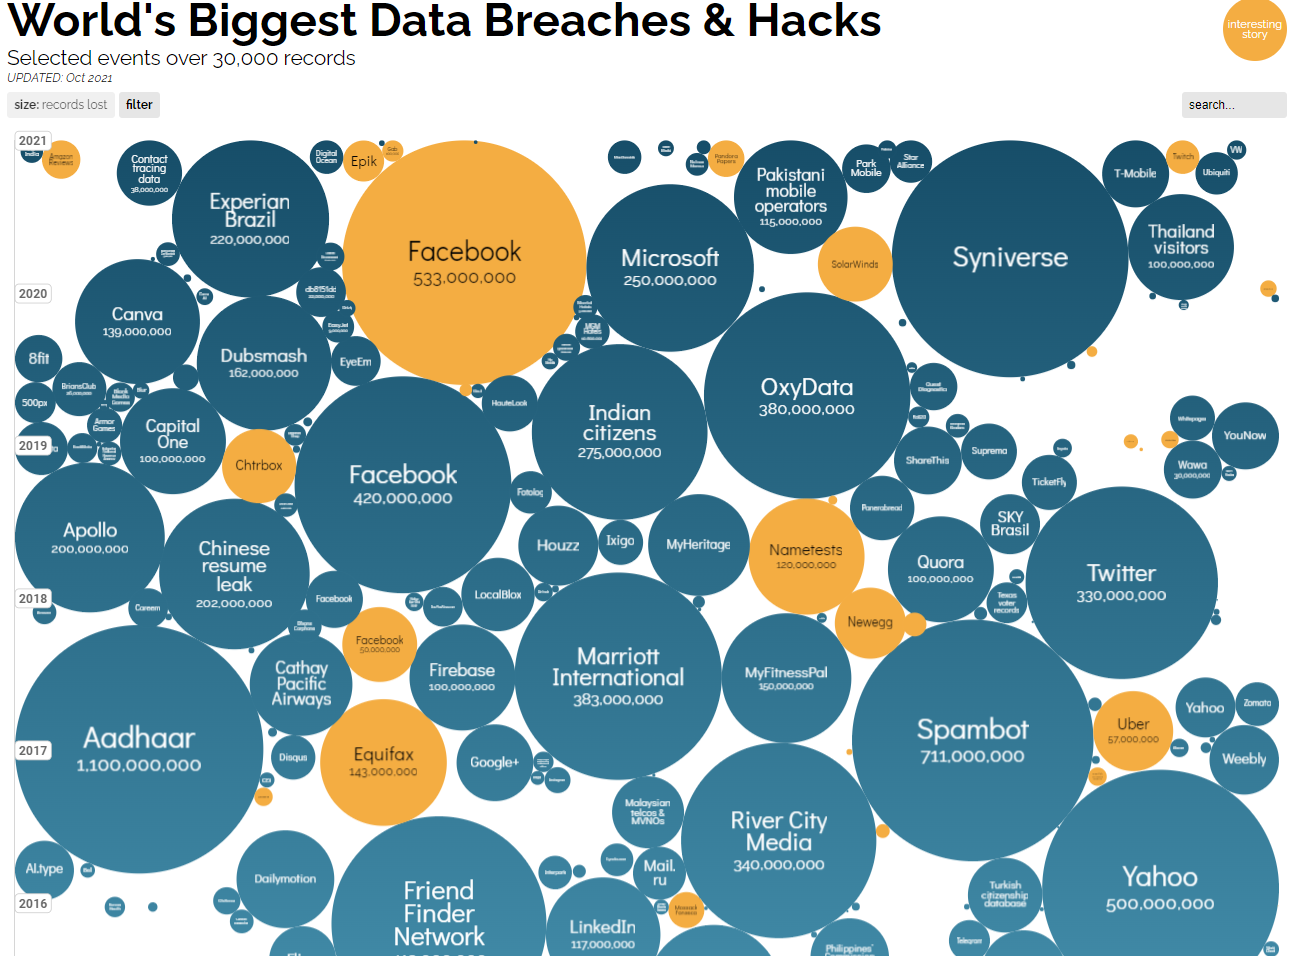
\includegraphics[width=8cm]{img/DataBreach.png}
s\caption{Word's Biggest data breaches and hacks occurred fro 2016 to October 2021  \cite{WorldDataBreach:online}}
\end{center}
\label{fig:worldDataBreach}
\end{figure}
Moreover, in 2021 several Nordic companies were victim of important cyber attacks ,peaking in December 2021\cite{Nordicco81:online}. Affected industries corresponded to the region’s largest industrial, food and  service providing sector.
Affected companies were Vestas, Wind Systems, Amedia, Nortura and Nordic Choice Hotels

\subsection{Hypothesis}
With the implementation of a decentralized system in a Hyperledger Fabric and
a chaincode implementing ERC-721 standard with IPFS network, it will be possible to manage and handle data between organizations in a safer and more secure
way. Sharing information and ensuring that the non-repudation10 principle remains consistent over the network no matter how many parties or users join the
infrastructure.


\section{Proposed Solution}
Having proposed the hypothesis to solve inter-organization data sharing and transmission through secure channels, the implementation of the system is shown in this section.

\subsubsection{System technologies}
The system gathers different technologies for the simulation 

\begin{figure}[ht]
    \centering
    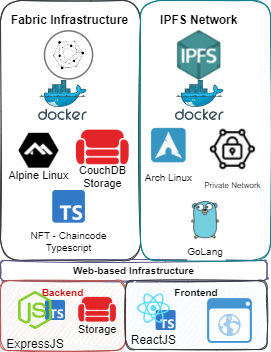
\includegraphics[width=7cm]{img/System-Technologies.png}
    \caption{System technologies used}
    \label{fig:SystemTechUSed}
\end{figure}

\begin{itemize}
    \item \textbf{Docker}. Set of platform as a service products that use OS-level virtualization to deliver software in packages called containers.
    \item \textbf{Hyperledger Fabric version 2.2} is used in the system. It uses Docker technology to run and simulate the system. it uses \textbf{Alpine Linux} as the OS repository.\cite{HyperledgerFabric:online}
    \item \textbf{Typescript}. A programming language superset of JavaScript developed and maintained by Microsoft. This code was used to develop the chaincode, back-end and front-end systems.
    \item \textbf{ExpressJS}. Back-end web application framework for Node.js designed for building web applications and APIs.
    \item \textbf{React}. Open-source front-end JavaScript library for building user interfaces based on UI components.
    \item \textbf{Apache CouchDB}. NoSQL document-oriented open-source database.
    \item \textbf{IPFS}\cite{benet2014ipfs}. Decentralized file storage system used content-addressed capabilities configured as a private network. It has been built in \textbf{GO} language and  \textbf{Alpine Linux} as OS. Uses \textbf{Docker} containers as a base image.
\end{itemize}


\subsubsection{Proposed architecture}
The components configured and assembled to integrate the infrastructure work in a Docker system.

\begin{figure}[ht]
    \centering
    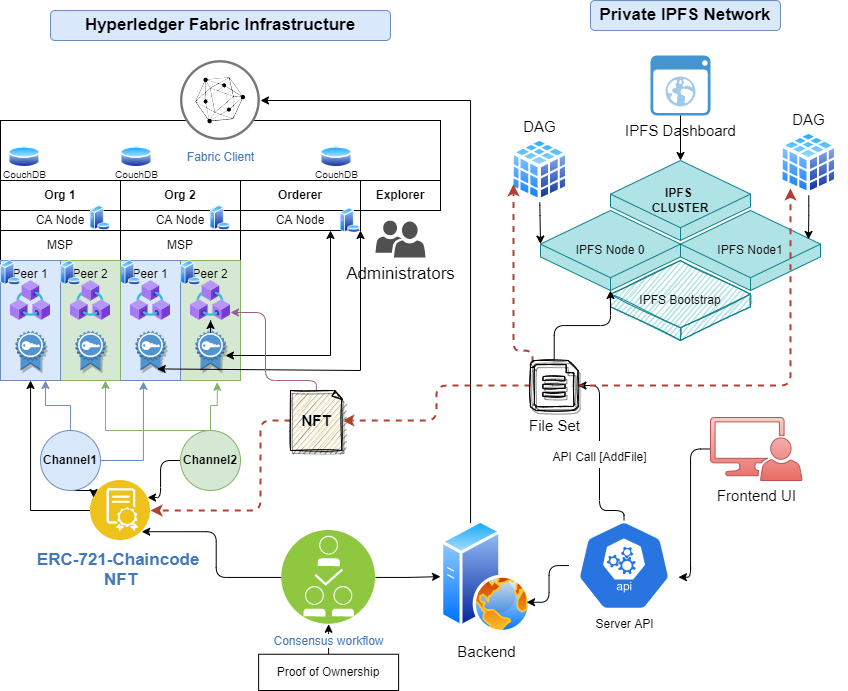
\includegraphics[width=9cm]{img/Hyperledger-NFT-Architecture.png}
    \caption{Proposed Architecture}
    \label{fig:SystemArch}
\end{figure}

\begin{itemize}
    \item \textbf{Hyperledger Fabric}. A a set of shell scripts and docker files assemble the required infrastructure to build the  DLT. The Fabric infrastructure has the following subcomponents: 
    \begin{enumerate}
        \item Organizations. Two organizations have been created. One organizations is build primarily to simulate the minting process of a NFT whereas the other can receive the minted token. The same process can also be made in the opposite way.
        \item Orderer node. Is the node in charge of sorting the transaction and creating the block. Once the block is created, it is forwarded to one of the organizations holding the Blockchain ledger. The orderer node does not hold a copy of the ledger but just coordinates and distributes the issued transactions.
        \item Orderer CA. Is the node in charge of issuing and validating the certificates of the organizations and the wallet creation (based on the root certificates) for the users to interact with the system.
        \item Channel. Organizations in Hyperledger can join and interact through a private channel. The channel is previously known by the two organizations and they participate by having a server that holds a version of the ledger, a database server and a certificate authority server.
        \item Chaincode. The smart contract used to manage the ledger transaction and mint digital assets as NFTs.
    \end{enumerate}
    \item \textbf{Private IPFS network}. Consists of a set of Docker containers where each system holds a copy of the IPFS file system\cite{benet2014ipfs}.
    \begin{itemize}
        \item IPFS bootstrap node. In the same way as the Ordered node receives the blocks of a transaction and transmits it to the organization nodes, it receives the file or data and transmits it to all the interconnected nodes, ensuring data persistence among the network.
        \item IPFS Dashboard. It works as the UI of the private network. Provides insights and data about the stored files and a preview of the data once a user can access through its content.
        \item IPFS Nodes. Each organization can contribute to the system data repository by holding an IPFS server.
    \end{itemize}
    \item \textbf{Back-end}. Server application that communicates with the Hyperledger network and extends its functionality by an API. 
    \begin{itemize}
        \item Connects organizations and corporate databases
        \item Communicates with the CA servers to issue and hold certificates.
        \item Communicates with IPFS private network API. 
        \item Holds a public REST API that provides all the functionality to register organizations, enroll users and mint NFTs.
        \item Interacts with the Blockchain smart contract and retrieves the information contained in the ledger. 
    \end{itemize}
    \item \textbf{Front-end}. It serves as the UI for user interaction. Allows the simulation of the system where any user can create an organization, enroll users, mint a NFT and visualize them in the list.
\end{itemize}



\section{Evaluation}

To simulate the system functionality a case for two persons from different organizations trying to issue and mint data, send it and making it available to one another.

\subsection{Setup and Scenario}
Simulation of two organizations willing to share data with each other.
\subsubsection{Organization 1}
Represents an organization with important information gathered from external resources, expensive and difficult to obtain. Has the technology and infrastructure to generate data, but does not count with the know how neither infrastructure to process it or exploit it (similar to machine learning / big data scenarios).

\textbf{User 'Minter'}
"Organization 1" Creates a user "Minter" as a company representative in charge of submitting the data and creating a NFT version of it inside the system. Then he can use the system to lend the data, enable a time frame visualization or transfer it.

\subsubsection{Organization 2}
Represents a technology company with skillful personal in data processing and domain area in the business of "Organization 1", but does not have the experience nor technology to gather it. Therefore it needs data from the aforementioned organization in order to create and expand their business.

\textbf{User 'Receiver'}
"Organization 2" Creates a user "Receiver"  as a company representative in charge of getting access to the NFT minted data by "Organization 1" via user "Minter" which will be used as the data source to perform machine learning training operations. 

With the use of the NFT System framework these parties can cooperate and participate by trusting that the information is secure, has not been altered and can be easily verified by them and other parties.

\section{Results}
The complete simulation of the process is shown in this section.

\subsection{System registering and user enrollment}
The NFT system provides a friendly user interface to allow organizations to be registered into the Fabric network to use a specific channel. 
Prior to this process Fabric generated a CA with which they can identify as trusted entities and fair participants of the network.

The first time an organization registers itself to join a private channel, an admin account is created. The admin account then is able to configure organization parameters and new users with restricted access or different mining/system-usage capabilities.
in the figure \ref{fig:SeqDiag_RegisterEnroll} can be visualized the process any organization will take to register itself as a valid participant with its corresponding representatives.

 \begin{figure}[ht]
        \centering
        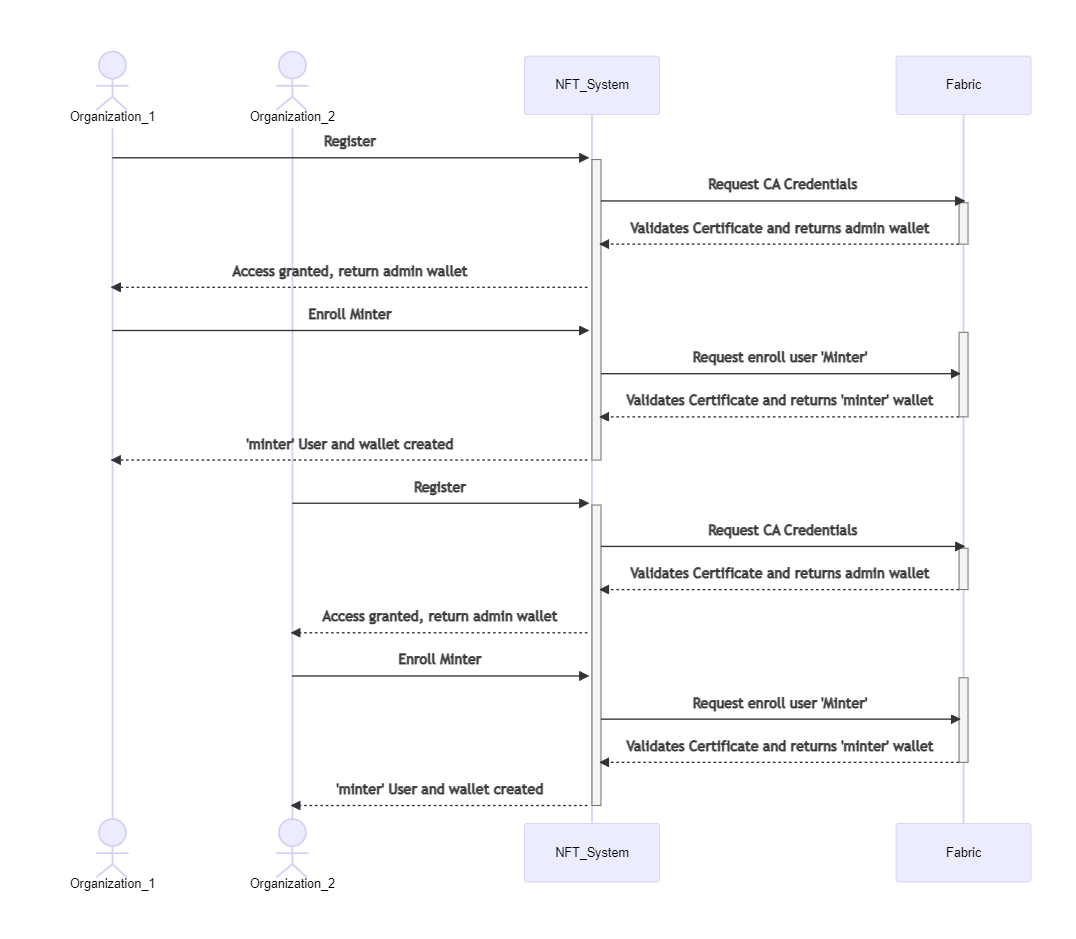
\includegraphics[width=8cm]{img/SequenceDiagram_RegisterEnroll.png}
        \caption{Sequence diagram of the Organization and user enrollment process in the system.}
        \label{fig:SeqDiag_RegisterEnroll}
    \end{figure}


 \begin{figure}[ht]
        \centering
        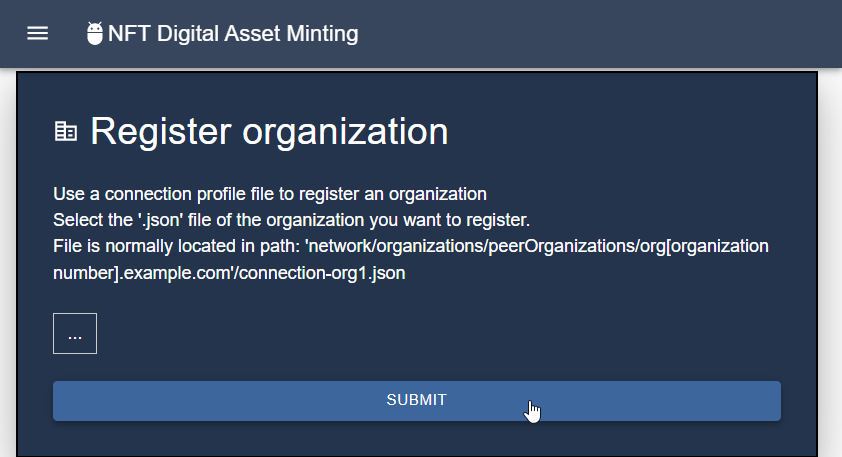
\includegraphics[width=7cm]{img/NFT_REGISTER.png}
        \caption{UI Register organization.}
        \label{fig:UI_Register}
    \end{figure}


 \begin{figure}[ht]
        \centering
        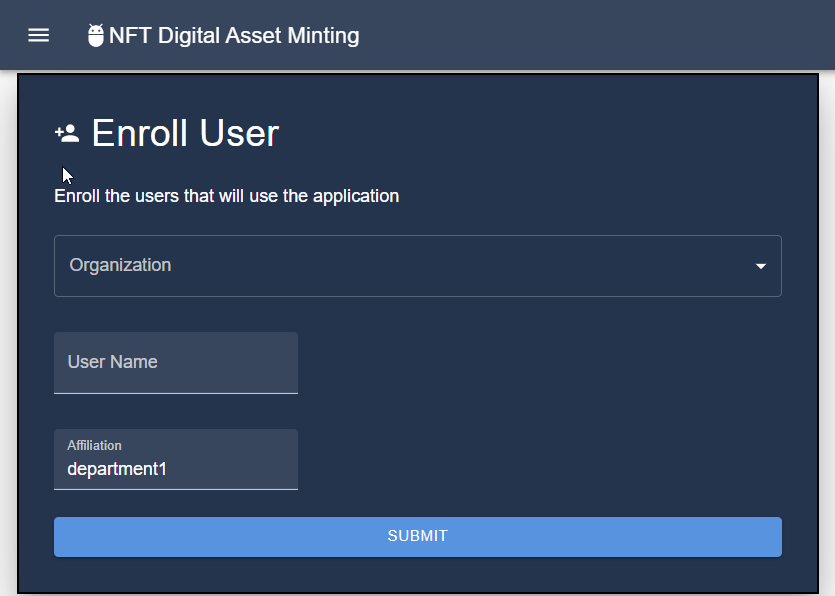
\includegraphics[width=7cm]{img/NFT_ENROLL.png}
        \caption{UI Enroll Users.}
        \label{fig:UI_Enroll}
    \end{figure}

\hfill \break

\subsection{NFT Minting and data reading access}
Once the organizations and users have been properly enrolled it the following steps must occur:
\begin{enumerate}
    \item Minter access to the platform and selects the "Mint 
    NFT option.
    \item Minter selects a file and completes the form metadata.
    \item Minter clocks on "submit" button to create the token.
    \item The System talks verifies that the file does not exist yet by:
    \begin{itemize}
        \item Asking to add the data file to the IPFS network
        \item Asking to Fabric if there is any token with the corresponding CID
    \end{itemize}
    For any of those cases to be true, the token will not be generated and an error will be returned.
    \item Once everything is approved the token is stored in the DLT with the corresponding file CID generated.
    \item 'Minter' can now send the CID or additional token information to 'Receiver'. Then receiver can pull such information from the infrastructure. Because of its unicity purposes 'Receiver' will not be able to counterfeit or take ownership of the data unless explicitly stipulated and agreed by both parties.
\end{enumerate}

 \begin{figure}[ht]
        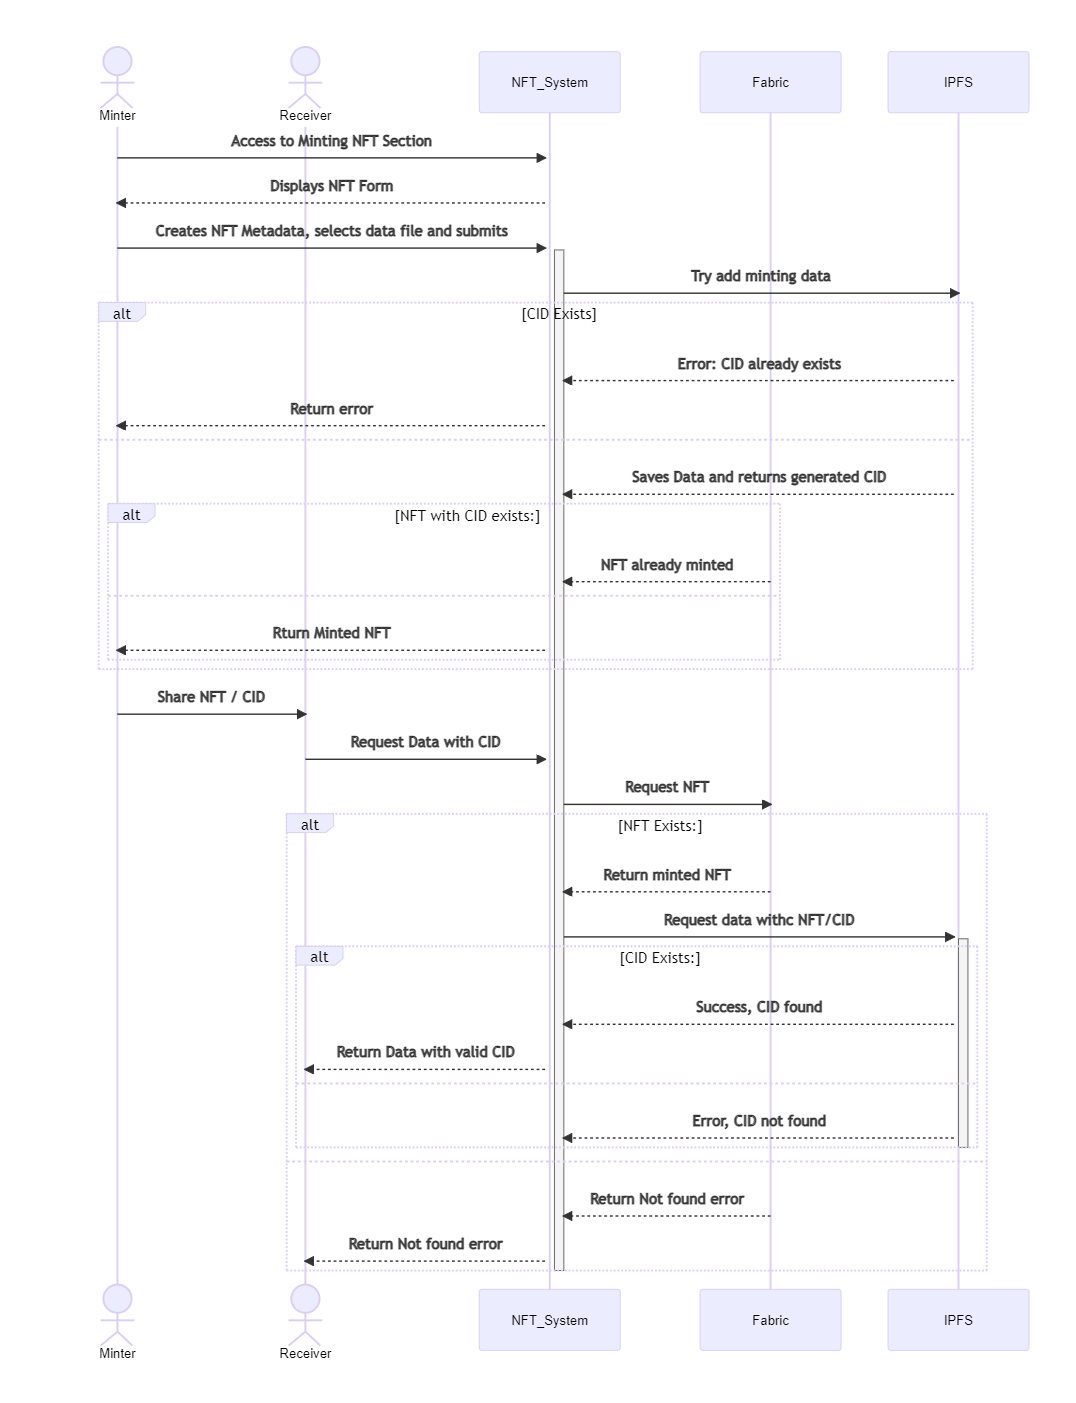
\includegraphics[width=8cm]{img/SequenceDiagram_MintNFT.png}
        \caption{Sequence diagram to mint a NFT}
        \label{fig:SeqDiag_Mint}
    \end{figure}
    
 \begin{figure}[ht]
        \centering
        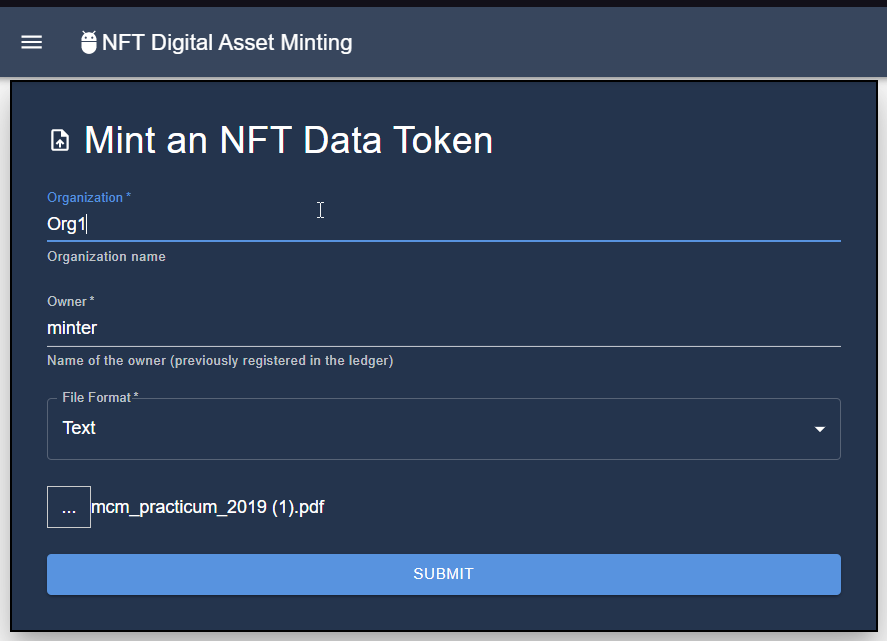
\includegraphics[width=6cm]{img/UIMinting.png}
        \caption{Front-end showing minting process.}
        \label{fig:UI_Mint}
    \end{figure}

 \begin{figure}[ht]
        \centering
        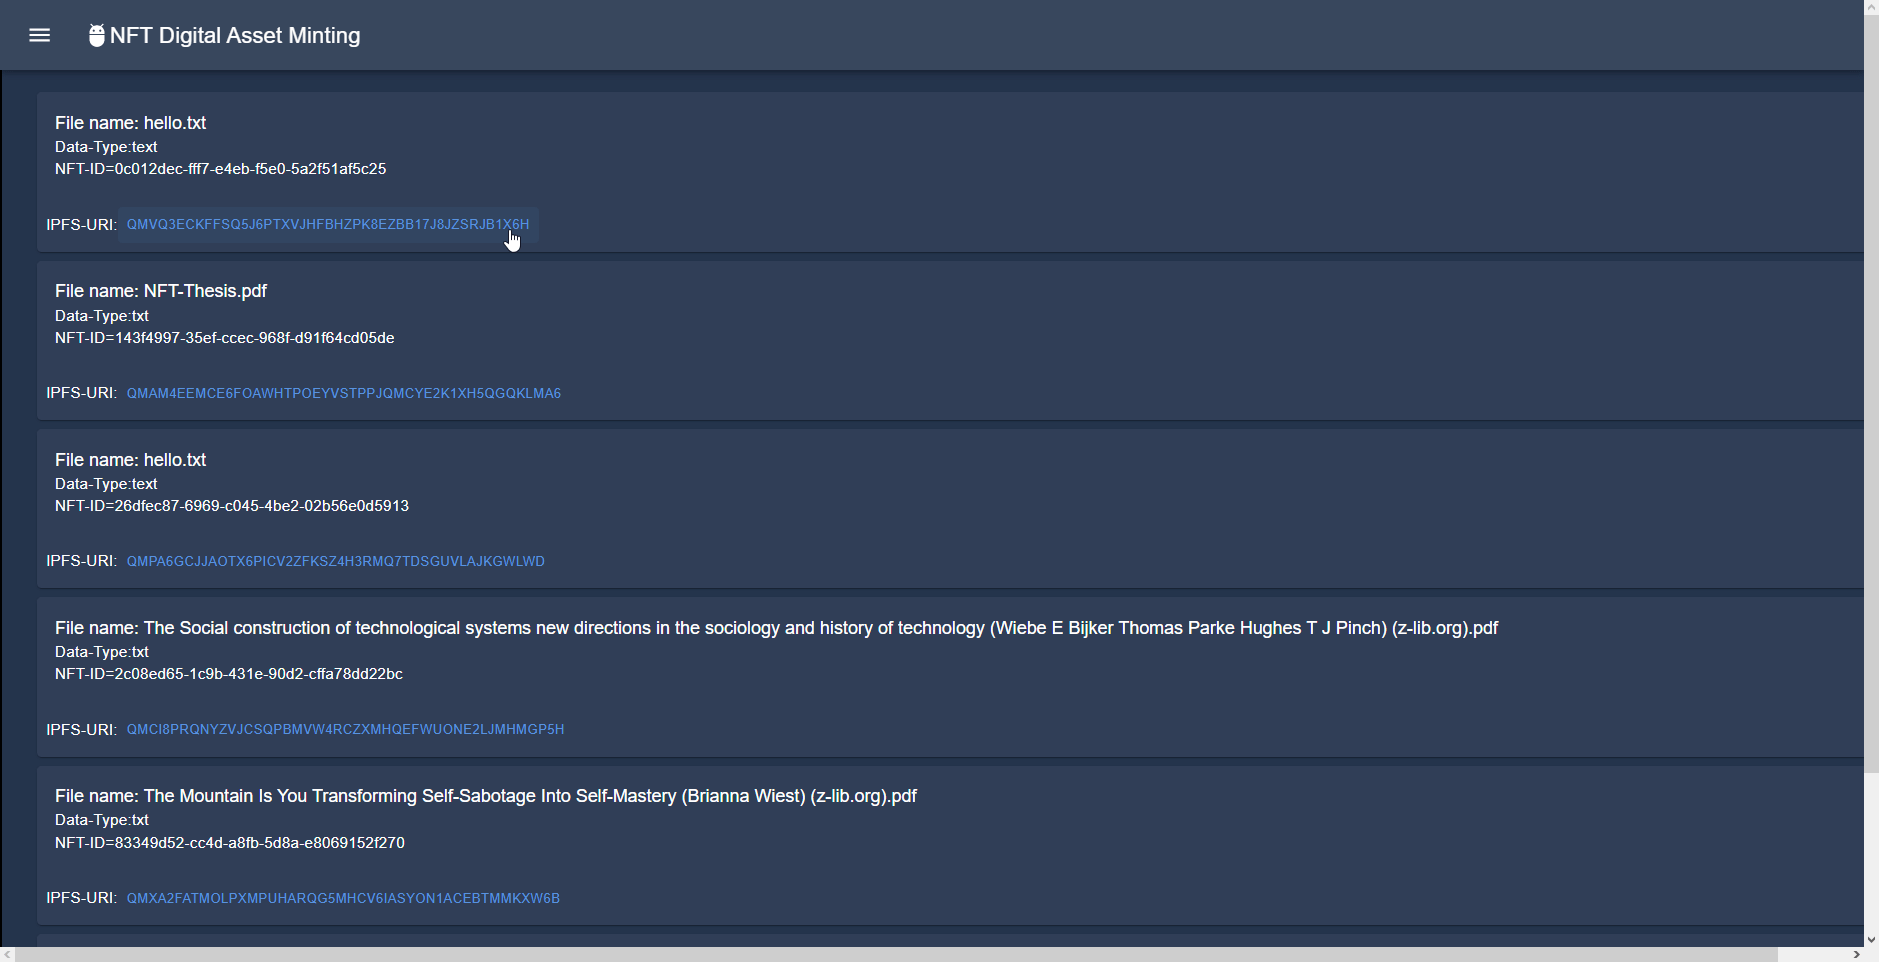
\includegraphics[width=7cm]{img/SystemList.png}
        \caption{Front-end showing minted NFTs in the system.}
        \label{fig:UI_MintTokens}
    \end{figure}
    
\subsection{NFT Transfer}
It is possible through the REST API to transfer the generated tokens from one owner to the other. This process will acknowledge that the new user is the new owner of the NFT. It is possible then to track the chain of ownership.

\subsection{NFT Burning}
The system also supports burning an NFT, which basically blocks the token and flags it as unusable. if that happens, burned NFT and CID data cannot be accessed via the platform.

IT is possible, however to access the data via the IPFS server.


\section{Discussion}


The implementation of digital asset management through issuance of NFTs represents a milestone in the generation of decentralized secure frameworks for industrial applications.

The implicit security of Blockchain with Hyperledger management and the privacy such technology offers will allow different organizations to participate and cooperate securely, but not anonymously. 

All parties will be able to acknowledge data ownership. If desired, data could be encrypted as well and managed trough additional smart contracts. In addition to this, IPFS network is able to control, distribute and manage the added data as a DFS. The final simulation of the environment allows testers, to acknowledge the workflow of the framework and further expand its capabilities in a modular way.

\section{Results}
The simulation was performed with the following operations:

\begin{enumerate}
    \item Minting NFT with Text data ~ 10KB
    \item Minting NFT with Image data ~ 200KB
    \item Minting NFT with Bin data ~ 100MB
    \item Minting NFT with a file of ~850MB
\end{enumerate}

The highest resource consuming process for the system is whenever data with high space resources is about to be minted. The communication with the server and IPFS network create a bottle neck in the simulation process and by running the resources locally.

\begin{table}[ht]
\begin{center}
\begin{tabular}{ |c|c|c|c|  }
 \hline
 \multicolumn{4}{|c|}{NFT Statistics} \\
 \hline
 No & File type & Size  & Elapsed time (s)\\
 \hline
 1   & Text     & 10KB &   0.5  \\
 2   & Image    & 200KB &   1.3 \\
 3   & PDF      & 100MB &   8.3 \\
 4   & Bin      & 850MB &   $\infty$ \\
 
 \hline
\end{tabular}
\caption{NFT Statistics.}
\label{table:NFTStats}
\end{center}
\end{table}

Whenever trying to mint an NFT File larger than 500 MB (previous tests were made with other files) the blockchain system, or at least the API server takes significantly larger amount time than expected to submit the data. Although this might be a parameter or server side configuration, it certainly refrains users from submitting large amounts of information.

Final results of the built application indicate that it is potentially feasible to create decentralized systems specialized in data management and control for industrial purposes while dealing with chunks of data. For text data it is relatively easy to mint, submit and visualize under the IPFS Server.

\subsection{Infrastructure statistics}
The following statistics were performed by running \textit{docker stats} command where they where later on plotted.
\begin{figure}[ht]
        \centering
        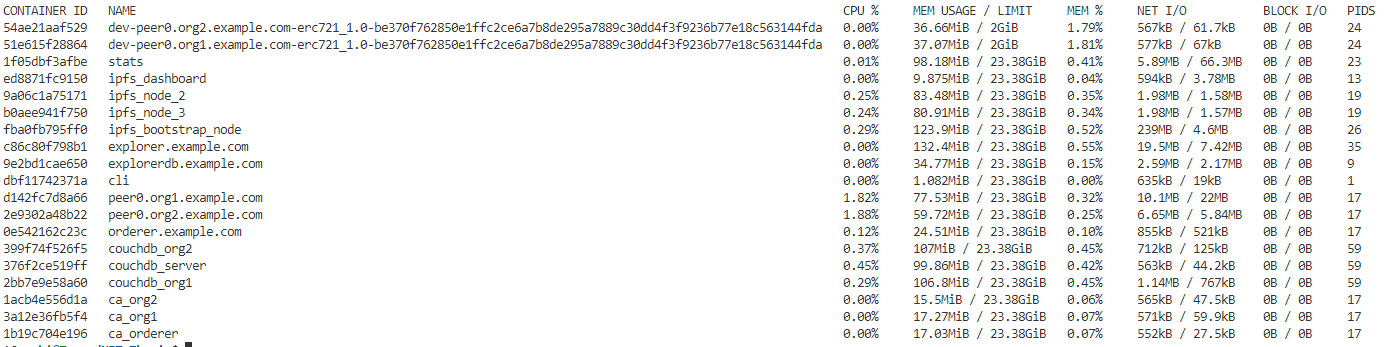
\includegraphics[width=7cm]{img/Docker_Stats.png}
        \caption{Docker statistics from current containers}
        \label{fig:dockerStats}
\end{figure}

\subsection{Benchmarking and Blockchain metrics evaluation}
Hyperledger framework has a benchmark tool used to measure the performance and behavior of the blockchain, test it and evaluate it under stress scenarios to check its latency and behaviour under heavy usage. Tables \ref{table:Benchmark1} and \ref{table:Benchmark2} show the results thrown in raw data. Figure \ref{fig:CaliperBenchmark} presents relevant information about the usage and network stress results. as an HTML report, which is also available at:
\url{https://htmlpreview.github.io/?https://raw.githubusercontent.com/asahicantu/NFT-Thesis/main/caliper-benchmarks/report.html} Units of measure for the data are in s and TPS.

\begin{table}[ht]
\begin{center}
\begin{tabular}{|p{2.1cm}|p{0.6cm}|p{0.4cm}|p{1.5cm}|p{1.5cm}|  }
 \hline
 \multicolumn{5}{|c|}{Blockchain benchmark Part I.} \\
 \hline
 Name & Succ  & Fail  & Send Rate (TPS) & Max Latency(s)\\
 \hline
 MintNFT.           & 5000   & 0 &   15.0  &  2.19  \\
 Query all NFTS.    & 9819   & 0 &   338.2 &  0.06 \\
 \hline
\end{tabular}
\caption{Blockchain Benchmark using Hyperledger Caliper Part I.}
\label{table:Benchmark1}
\end{center}
\end{table}

\begin{table}[ht]
\begin{center}
\begin{tabular}{ |p{2.1cm}|p{1.2cm}|p{1.5cm}|p{1.5cm}|  }
 \hline
 \multicolumn{4}{|c|}{Blockchain Benchmark using Hyperledger Caliper Part II.} \\
 \hline
 Name & Min Latency (s) & Avg Latency (s) & Throughput (TPS)\\
 \hline
 MintNFT.        & 0.10  & 0.43 & 14.9 \\
 Query all NFTS. & 0.01  & 0.02 & 338.1 \\
 \hline
\end{tabular}
\caption{Blockchain Benchmark using Hyperledger Caliper Part II.}
\label{table:Benchmark2}
\end{center}
\end{table}

 \begin{figure}[ht]
        \centering
        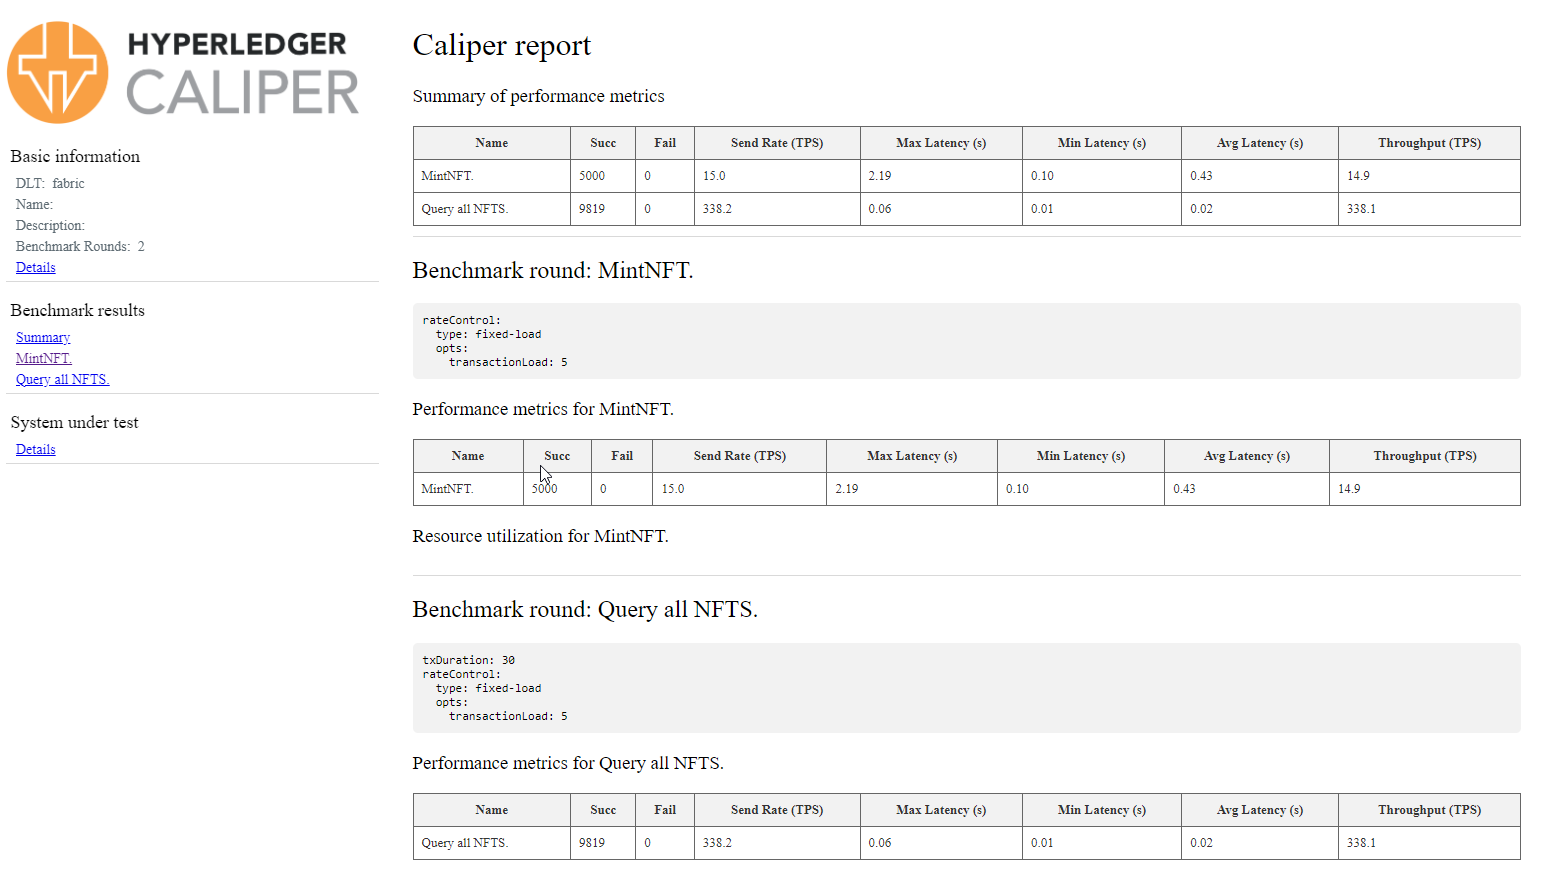
\includegraphics[width=7cm]{img/Caliper.png}
        \caption{Hyperledger Caliper Benchmark results.}
        \label{fig:CaliperBenchmark}
    \end{figure}

\section{Conclusions}

In line with the original hypothesis it is possible to confirm that the construction of decentralized systems is possible and will create yet unforeseen possibilities to manage information and provide:
\begin{itemize}
    \item System scalability
    \item Modularity
    \item Self Governance by smart contract agreement
    \item Privacy and security
    \item Mutual cooperation
\end{itemize}

Systems such as this can be governed or not by a central authority. Depending on the business needs and industrial purposes different scenarios could be developed and simulated.

Key findings through the research and development of this project are:
\subsection{Blockchain and DLT}.
Data integrity and consistency safeguarding. Decentralized system nowadays allow very easily to verify data origin, integrity and non-repudation principle  establishes new ways of working and contributing for the development and research of technology.

\subsection{Security}
The created infrastructure has several layers of security and implicit elements to protect parties and their data from improperly accessing information. 
\subsubsection{CAs}
Different parties can choose to rely over a central or multiple CAs. As long as there is a common agreement previously established by smart contracts and common consensus, it will be possible to create highly resistant and resilient systems to malicious attacks. The modularity of Blockchain allows the cooperation of parties in benefit of the whole system, therefore rejecting undesirable or suspicious behaviour.

\subsubsection{Private channels}
Private channels in Hyperledger Fabric allow organizations to create a subsystem inside the framework, where sub smart contracts can be created to allow privacy between a single, two or more entities in different regions of the world.
Therefore, while every organization can hold a copy of the ledger and data, only those with the right privileges can be allowed to interact with the hidden rules.

IPFS offers several layers of security, data can be encrypted and directed by smart contract instructions and even by the security layers set into the built system. 

\subsection{Governance}
Organizations can self in their best interest to preserve business functionality and choose the most suitable way to manage data. That being said, they will be able to choose which CA is the best, what rules in the smart contract can be implemented and under which conditions entities can mint or transfer NFTs.


\section{Future Work}
It is intended for anyone willing to extend and expand the functionality of this work to move within the following points:
\subsection{System integration}
This project can complement the work made by \cite{akbarAli}, which explains how shared data can be used to perform workflows for different purposes such as Big data analytics and Machine learning. One key advantage of this implementation relies on the fact that participants will have no direct access to shared data itself, but to a framework where it can be processed and manipulated to generate different models and insights. When connecting both systems, it will be possible to create and encapsulate information, self data encryption can grant that even different organizations own a copy of the blockchain and IPFS network, they cannot read the information unless they do it directly from the proposed application.

\subsection{NFT and Smart Contract extension}
An extension of ERC-721\cite{ERC721No30} smart contract implemented can be easily extended to create new business rules such as:

\subsubsection{NFT delegated ownership and transfer}
Not only one user, but multiple entities could possess a digital asset, sharing a percentage of such element. Therefore new rules can be suggested to interact, protect and manipulate information.

\subsubsection{Consensus}
New consensus mechanisms can be generated to incentivize the usage of the network. This project contains for example rules to rank information and create a reputation level for the organizations, which can increase the value of the minted NFT. In other scenarios can be possible to create digital ownership by data origin, geographical location and mechanisms of burning so it cannot be used by other parties.
 
\subsubsection{Economics through Tokenization}
A very interesting approach to explore is the creation of economic tokens integrated with the NFT system. Such tokens and in the same form that ETH does with the Ethereum platform, every piece of data can be linked to another unity of tokens where once transferred its value in tokens can be transferred as well. The token-value of data can increase as its ranking of "valuable information" increases, or organization reputation does.
Depending on those economic mechanisms, different companies could be able to generate royalties and incentivize the usage of the system. Furthermore.

\subsubsection{Multi-system integration}
Furthermore, this project can be integrated with other public Blockchain platforms, and allow the issuance or reading of  Ethereum smart contracts, enabling its execution in the internal network. The possibilities are endless and adaptable to specific business needs.


\section{Code and Instructions}
\label{apx:main}

\section{File repository}
\label{FileRep}
The repository with the code to download the system and perform the simulation is available at:
\url{https://github.com/asahicantu/NFT-Thesis}.
The repository file includes a video sequence showing the steps to perform a simulation and code run.

%
\newpage
 \bibliographystyle{abbrv}
  \bibliography{Bibliography}  % The references (bibliography) information are stored in the file named "Bibliography.bib"


\end{document}
